\chapter{Grundlagen und Technologien}
\label{cha:StandDerTechnik}

In diesem Kapitel werden die grundlegenden funktionalen Testmethoden beschrieben, welche in der Softwareentwicklung angewendet werden. Andere Testbereiche der Softwareentwicklung wie Performanztest und Penetrationstest werden hier nicht behandelt, denn die vorliegende Arbeit zielt speziell auf die funktionalen Testmethoden ab und hat in diesem Bereich ihre Stärken, was aber nicht bedeutet, dass man dieselben Konzepte nicht auch für die anderen Testbereiche anwenden könnte. 


\begin{figure}
\centering
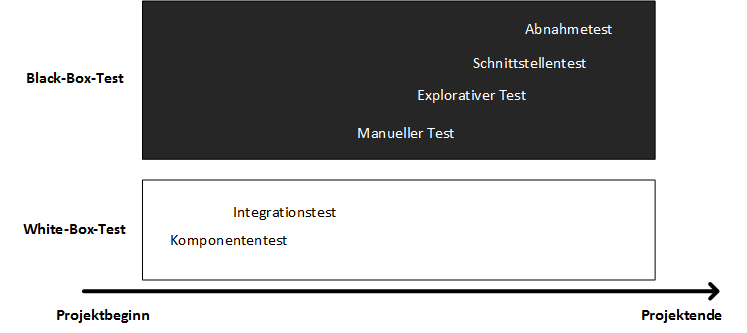
\includegraphics[width=0.9\textwidth]{testuebersicht.png}
\caption{Testmethoden unterteilt in \enword{White-Box-} und \enword{Black-Box}-Testen}
\label{fig:testtypen}
\end{figure}

\SuperPar
Funktionale Tests haben die Aufgabe sicherzustellen, dass die Anforderungen aus der Spezifikation korrekt umgesetzt werden. Für die Umsetzung dieser Tests können sowohl manuelle als auch automatisierte Testmethoden verwendet werden, welche in Abbildung \ref{fig:testtypen} dargestellt sind. Die unterschiedlichen Methoden werden in diesem Kapitel genauer beschrieben und es wird auf die Unterschiede eingegangen.

\SuperPar
Im zweiten Teil dieses Kapitels werden die verwendeten Technologien beschrieben. Dazu gehören die Werkzeuge und Bibliotheken, welche für die Entwicklung von Rayden verwendet werden. Diese Werkzeuge und Bibliotheken werden benötigt, da Rayden aus einer Sprache, Compiler, Interpretierer und weiteren Komponenten besteht. Weiters werden zwei Testtreiber-Bibliotheken beschrieben, welche für automatisierte Abnahmetests verwendet werden können. 

\section{\enword{White-Box}-Test}

Unter \enword{White-Box}-Tests versteht man Tests, bei denen die Testerinnen und Tester Zugriff auf den Quelltext haben. \enword{White-Box}-Tests werden speziell für bestimmte Codefragmente geschrieben und testen gezielt einzelne Teile einer Anwendung. Diese Tests werden in einer frühen Phase des Entwicklungsprozesses erstellt und liefern sehr bald Qualitätskennzahlen. 

\SuperPar
Diese Tests sind typischerweise sehr technisch und verlangen vom Testpersonal Programmierkenntnisse. Daher werden diese Tests von Personen aus der Entwicklungsabteilung selbst geschrieben und fallen nicht in den Zuständigkeitsbereich des Qualitätssicherungsteams. Das gilt natürlich nur solange, als man sich nicht in einem agilen Entwicklungsprozess befindet. Dort werden sowohl die \enword{White-Box}- als auch die \enword{Black-Box}-Tests im Entwicklungsteam umgesetzt.


\section{\enword{Black-Box}-Test}

Die \enword{Black-Box}-Tests sind klassische Aufgaben eines Qualitätssicherungsteams. Sie umfassen alle Testansätze, bei denen der Quelltext der Anwendung nicht vorliegt. Dabei ist die Anwendung also eine \enword{Black Box}. Die Aufgabe des Qualitätssicherungsteams ist es, zu überprüfen, ob alle Anforderungen laut Spezifikation umgesetzt wurden. Für diese Aufgabe steht dem Qualitätssicherungsteam eine ganze Reihe an unterschiedlichen Ansätzen zur Verfügung, angefangen von manuellen Tests über explorative Tests bis hin zu automatisierten Abnahmetests. 

\SuperPar
Die \enword{Black-Box}-Tests werden typischerweise im fortgeschritten Projektstadium durchgeführt. Das ergibt sich aus der Tatsache, dass man für die \enword{Black-Box}-Tests eine lauffähige Anwendung benötigt.

\section{Manuelle Testmethoden}

Bei manuellen Tests handelt es sich generell um \enword{Black-Box}-Tests. Dabei überprüft die Testerin oder der Tester, ob sich die Anwendung in Bezug auf die in der Spezifikation angegebenen Anforderungen korrekt verhält und ob die Funktionalität vollständig vorhanden ist. Die Funktionalität wird typischerweise über die Benutzeroberfläche geprüft. Eine zusätzliche Aufgabe bei manuellen Tests ist es, zu überprüfen, ob die Benutzeroberflächen-Konzepte korrekt und einheitlich umgesetzt wurden.

\SuperPar
Bei manuellen Tests ist es typisch, dass die Testmanagerin oder der Testmanager eine textuelle Beschreibung der Testfälle erstellt. Diese Testfälle werden dann von dem Qualitätssicherungsteam für jede neue Version der Anwendung durchgeführt. Bei einer Abweichung der Anwendung muss entschieden werden, ob sich der Anwendungsfall geändert hat oder ob die Anwendung nicht korrekt funktioniert. Im letzteren Fall muss ein Fehlerbericht verfasst und an die Entwicklungsabteilung gesendet werden.

%%\subsection{Explorativer Test}

\SuperPar

Eine Spezialform des manuellen Testens ist das explorative Testen. Dabei bekommt die Testerin oder der Tester keine genaue Vorgabe, wie ein Anwendungsfall getestet werden soll. In diesem Fall bekommt die Person nur eine Aufgabe gestellt, welche mit der Anwendung gelöst werden muss. Das Ziel ist es, dass man unterschiedlichste Möglichkeiten der Anwendung testen kann. Dieser Ansatz ist gut dafür geeignet, um neue Fehler zu finden. 

\SuperPar
Grundsätzlich haben manuelle und automatisierte Tests die Limitierung, dass nur festgestellt werden kann, ob eine neue Version einer Anwendung gleich gut funktioniert wie die alte. Es können aber keine neuen Fehler abseits der definierten Tests gefunden werden. Diese Lücke versucht das explorative Testen zu schließen. Es ist auch von Vorteil, wenn nicht immer die gleiche Person dieselbe Aufgabe testet. Jede Person hat neue Ideen, wie man die Aufgabe lösen kann und testet daher neue Bereiche und Kombinationen der Anwendung. Dieser Ansatz ist ein kreativer Prozess und kann daher im Gegensatz zu manuellen Tests nicht automatisiert werden.

\section{Automatisierte Testmethoden}

Das Ziel von automatisierten Tests ist es, dass man den Testaufwand in einem Softwareprojekt reduziert. Aus wirtschaftlicher Sicht ist es viel besser, wenn das stupide Testen durch einen automatisierten Test erledigt wird. Dadurch reduzieren sich die Kosten für das Softwareprojekt. Bei einer manuellen Ausführung kann es bei mehrmaligen Wiederholungen eines Tests zu Aufmerksamkeitsverlusten kommen, was bei automatisierten Tests nicht der Fall ist.

\SuperPar
Durch automatisierte Tests werden Qualitätssicherungsteams jedoch nicht obsolet. Auf der einen Seite müssen die automatisierten Tests auch von jemandem geschrieben und gewartet werden, auf der anderen Seite sind automatisierte Tests für exploratives Testen ungeeignet. Die Aufgabe des explorativen Testens wird auf absehbare Zeit immer durch Personen erledigt werden.

\SuperPar
Schlussendlich gibt es noch einen weiteren wichtigen Vorteil von automatisierten Tests gegenüber manuellen Tests: Man kann automatisierte Tests viel öfter ausführen und sie liefern schneller eine Aussage über die Qualität der Software. Diese Zeitreduktion ist für agile Softwareprozesse sehr wichtig, denn damit bekommt das Entwicklungsteam schneller eine Rückmeldung darüber, ob das System (noch) korrekt funktioniert. 


\subsection{Komponententest (\enword{Unit Testing})}

Bei einem Komponententest \cite{xUnit} wird genau eine Softwarekomponente getestet. Eine Softwarekomponente ist eine abgeschlossene Einheit in einem Softwareprojekt, welche eine definierte Schnittstelle hat. Das kann zum Beispiel eine einzelne Klasse, aber auch ein ganzes Modul sein, wie zum Beispiel in Pascal. Aus diesem Grund wird der Komponententest auch oft als Modul-Test oder Unit-Test bezeichnet. In dem Fall, dass die zu testende Komponente eine Abhängigkeit von einer anderen Komponente hat, werden diese durch eine Test-Implementierung ersetzt. Der Vorteil von Komponententests ist, dass deren Erstellung und Wartung keinen großen Aufwand verursachen. Das ist auch der Grund, warum dieser Testansatz sehr beliebt und weit verbreitet ist. Die Beliebtheit dieser Variante kann man daran ablesen, dass es mittlerweile für so gut wie jede Programmiersprache eine Unit-Test-Bibliothek wie zum Beispiel \enword{JUnit} \cite{JUnit} gibt. Der Vorteil ist aber auch der größte Nachteil bei diesem Ansatz: Die Komponenten werden einzeln getestet und man kann daher keine Aussage darüber treffen, wie sich das Gesamtsystem verhalten wird.

\SuperPar
Um eine Aussage über das Verhalten des Gesamtsystems zu erhalten, kann man Integrationstests verwenden. Diese werden im nächsten Abschnitt erklärt.

\subsection{Integrationstest (\enword{Integration Testing})}

Der Integrationstest ist schon deutlich aufwendiger und umfangreicher als ein Komponententest. Bei einem Integrationstest werden alle Komponenten eines Softwaresystems gemeinsam getestet. Das Ziel bei diesen Tests ist es zu gewährleisten, dass alle Komponenten miteinander funktionieren und dass alle Schnittstellen korrekt implementiert wurden. Es werden auch unterschiedliche Fehlersituationen im System simuliert und überprüft, ob diese ausgeglichen werden können. Ein einzelner Fehler in einer Komponente soll nicht das ganze System zum Absturz bringen oder in einen ungültigen Zustand versetzen.

\SuperPar
Bei einem Integrationstest stellt sich oft die Frage, ob man mit oder ohne Datenbank testen soll. Diese Frage kann man nicht so einfach beantworten. Auf der einen Seite kann man sagen, dass die Datenbank genauso eine Komponente im Softwaresystem ist, welche getestet werden muss. Auf der anderen Seite kann man argumentieren, dass die Datenbank ein externes System ist, welches bereits getestet wurde. Grundsätzlich ist jedoch zu sagen, dass es ein guter Ansatz ist, wenn man mit einer Datenbank die Integrationstests durchführt. Eine ausführliche Diskussion über diese Thematik kann man in \enword{Der Integrationstest} \cite{intTest} nachlesen. Es kann immer wieder vorkommen, dass genau bei der Schnittstelle zwischen Softwaresystem und Datenbank Probleme auftreten. Diese Fehler würden sonst erst relativ spät im Projekt-Lebenszyklus auftreten und der Aufwand für die Behebung dieser Fehler würde steigen.

\SuperPar
Der Grund, warum über dieses Thema so viel diskutiert wird ist, dass der Aufwand für einen Integrationstest mit Datenbank deutlich höher ist. Man muss eine Strategie finden, wie man für jede Testausführung einen definierten Datenbankzustand herstellen kann. Dieser Datenbankzustand ist sehr wichtig, um reproduzierbare Tests schreiben zu können. 


\subsection{Schnittstellentest (\enword{API Testing})}

Der Schnittstellentest ist die Vorstufe zum Abnahmetest, bei welcher alle externen Schnittstellen getestet. Dabei kann es sich um eine Schnittstelle zu einem externen System handeln oder um eine Web-Service-Schnittstelle. Aber darunter fällt auch die Schnittstelle zwischen Benutzeroberfläche und Geschäftslogik. Gerade diese Schnittstelle ist für die Testautomatisierung sehr interessant, da man hierbei die Benutzeroberfläche nicht für das Testen benötigt, jedoch das Gesamtsystem testen kann. Der Vorteil liegt darin, dass dieser Testansatz deutlich stabiler ist als ein Abnahmetest, welcher die Tests über die Benutzeroberfläche ausführt. Auch ist die Durchlaufzeit eines Schnittstellentests deutlich geringer als bei einem Abnahmetest.

\SuperPar
Der Unterschied zwischen einem Schnittstellentest und einem Integrationstest ist, dass bei einem Schnittstellentest das Software-System vollständig installiert wird. Für die Tests wird eine vollwertige Datenbank mit realistischen Testdaten verwendet. Bei einem Integrationstest verzichtet man auf diesen Aufwand.

\SuperPar
Wie schon die vorhergehenden Testansätze hat auch dieser Ansatz einen großen Nachteil: Bei diesen Tests werden nur die Schnittstellen zwischen externem System und der Benutzeroberfläche getestet. Dabei kann aber nicht sichergestellt werden, dass die Benutzeroberfläche fehlerfrei funktioniert. Für die Benutzerin oder den Benutzer der Anwendung zählt schlussendlich nur, ob die Verwendung über die Benutzeroberfläche korrekt funktioniert. Aus diesem Grund sind all diese Testansätze kein Ersatz für die Abnahmetests.

\subsection{Abnahmetest (\enword{User Acceptance Testing})}

Abnahmetests sind die aufwendigsten und kostenintensivsten Aufgaben im Testprozess. Bei einem Abnahmetest wird die Anwendung aus Sicht der Benutzerin oder des Benutzers getestet. Das Qualitätssicherungsteam verifiziert, ob alle Anwendungsfälle und Funktionen, welche in der Spezifikation definiert worden sind, vorhanden sind. Dafür muss eine lauffähige Anwendung vorhanden sein, um diese Tests durchführen zu können. Im Wasserfall-Vorgehensmodell kommt dieser Testansatz am Ende des Entwicklungszyklus. Es kommt dabei nicht selten vor, dass die Kundin oder der Kunde diese Tests manuell durchführt. Bei den agilen Vorgehensmodellen werden diese Tests nach jeder Iteration durchgeführt. Durch die kurzen Iterationszyklen können die Abnahmetests nicht mehr manuell durchgeführt werden. In diesem Fall kommen automatisierte Abnahmetests zum Einsatz. 

\SuperPar
Die große Herausforderung bei diesem Testansatz ist es, die Balance zwischen manuellen und automatisierten Tests zu finden.

\section{Verwendete Technologien}

Rayden basiert auf und verwendet eine Vielzahl von unterschiedlichen Technologien, Werkzeugen und Bibliotheken. Dieser Abschnitt gibt einen Einblick in diese Technologien und erklärt, in welchen Bereichen diese im Rayden-System verwendet werden. Als Basis wird die Programmiersprache \enword{Java} und deren Laufzeitumgebung verwendet. Die Entscheidung für \enword{Java} ist essentiell für das Projekt, um eine große Anzahl an unterschiedlichen Test-Szenarien zu unterstützen. 

\SuperPar
Für die Umsetzung der Sprache Rayden wurden viele Bibliotheken und Werkzeuge aus dem Eclipse-Umfeld verwendet. Als Testtreiber-Bibliotheken werden sowohl die offene Selenium- als auch die kommerzielle \enword{Borland Silk Test}-Implementierung verwendet.

\subsection{Eclipse}

Eclipse \cite{Eclipse} ist eine Entwicklungsumgebung für eine Vielzahl an Programmiersprachen. Ursprünglich wurde Eclipse von IBM für die Sprache \enword{Java} entwickelt. Im Laufe der Zeit wurde Eclipse zu einer beliebten Entwicklerplattform und es wurden immer mehr Sprachen über \enword{Plug-ins} unterstützt. Auch für das Rayden-System soll ein solches \enword{Plug-in} entwickelt werden, um eine gute Unterstützung bei der Erstellung von Tests bieten zu können. 

\SuperPar
Neben der Entwicklungsumgebung ist Eclipse aber auch eine Plattform für die unterschiedlichsten Projekte geworden. Diese Projekte werden von der \enword{Eclipse Foundation} \cite{EclipseFoundation} verwaltet und durch Partnerunternehmen und Freiwillige gepflegt. 

\SuperPar
Einige dieser Projekte werden in den nächsten Abschnitten separat vorgestellt.

\subsection{\enword{Eclipse Modeling Framework}}

Das \enword{Eclipse Modeling Framework} (EMF) \cite{EMF} ist ein Modellierungswerkzeug für \enword{Java}. EMF stellte eine Menge an Werkzeugen zur Erstellung, Verwaltung und Weiterverarbeitung zur Verfügung. Dazu gehört auch die Möglichkeit, aus diesen Modellen Code zu generieren. Eine Kernkomponente von EMF ist das ECore-Metamodell. Ein Metamodell ist die Schablone für ein spezifisches Modell. Aus einem ECore-Modell kann man mithilfe von Code-Generatoren eine \enword{Java}-Bibliothek generieren.

\SuperPar
Auf diesem Konzept baut auch das xText-Projekt auf, welches im nächsten Abschnitt vorgestellt wird. 

\subsection{xText}

Das xText-Projekt \cite{xtext} unterstützt das Erstellen von neuen Sprachen. Grundsätzlich ist xText ein Compiler-Generator der aus einer Grammatik einen lexikalischen und einen Syntax-Analysator generiert. Das Besondere an xText ist aber, dass man noch zusätzlich einen Eclipse-Editor für die Sprache bekommt. Der Editor bietet grundlegende Funktionen wie Syntax-\enword{Highlighting}, Fehler- und Validierungsmechanismen. Diese Funktionalität kann man nachträglich noch anpassen und weitere Funktionen hinzufügen. Ein Vorteil von xText ist, dass man den generierten Compiler auch außerhalb von Eclipse als eigenständige Anwendung verwenden kann. Somit kann der Aufwand, zwei Compiler für seine Sprache warten zu müssen, eingespart werden. Der abstrakte Syntaxbaum einer Quelldatei wird im Compiler mit EMF umgesetzt. Das heißt, man bekommt einen vollständigen Syntax-Baum im Hauptspeicher, welchen man sehr einfach verarbeiten kann. Um die Verwendung noch zu vereinfachen, liegt für den Baum ein Metamodell in Form eines ECore-Modells vor. 

\subsection{Selenium}

Selenium \cite{Selenium} ist eine Open-Source-Bibliothek, um Web-Seiten automatisiert testen zu können. Die Bibliothek unterstützt eine Vielzahl an unterschiedlichen Browsern auf allen gängigen Betriebssystemen wie Windows, Linux, Macintosh und Google Android. Um die Browser ansprechen zu können, benötigt man einen speziellen Treiber. Dieser wird entweder als separate Anwendung aus- oder bereits mit dem Browser mitgeliefert.

\SuperPar
In der ersten Version hat Selenium auf eine proprietäre Programmierschnittstelle gesetzt. Seit der Version 2 setzt Selenium auf die standardisierte Programmierschnittstelle \enword{WebDriver} \cite{WebDriver} des W3C Konsortiums. Der Vorteil von \enword{WebDriver} ist, dass man eine einheitliche Programmierschnittstelle für die unterschiedlichsten Browser hat. Damit erzielt man Unabhängigkeit von einem spezifischen Browser. 

\subsection{Borland Silk Test}

\enword{Borland Silk Test} \cite{SilkTest} ist eine kommerzielle Testsoftware für native wie auch Web-Anwendungen. \enword{Silk Test} bietet Unterstützung für eine Vielzahl an unterschiedlichen Technologien. Unterstützt werden zum Beispiel die gängigen Browser wie Internet Explorer, Google Chrome und Mozilla Firefox. Neben Web-Technologien werden auch native Windows-, Adobe-Flex-, Windows-Presentation-Foundation- oder \enword{Java}-Anwendungen unterstützt. Seit kurzem werden auch Browser und Anwendungen  auf mobilen Geräten unterstützt. Der Vorteil von \enword{Silk Test} gegenüber von Selenium ist, dass es einen verbesserten \enword{X-Browser Support} gibt. Dabei kann man einen Test, welchen man zum Beispiel mit dem Internet Explorer aufzeichnet, mit einem Mozilla-Firefox- oder dem Google-Chrome-Browser ausführen. Durch diese \enword{X-Browser}-Technologie entfällt die Wartung von Tests für die verschiedenen Browser. 
